Comme expliqué dans la partie Planning, nous avons prévu une réunion client chaque semaine, ainsi que une réunion industriel. En général, les réunions industriels sont prévues en début de semaine,
et les réunions clients le vendredi pour nous permettre de mettre en place la méthode "scrum" évoquée précedemment. La réunion industielle est placée ainsi pour permettre en début de semaine de prévoir la semaine
à venir : on peut ainsi prévoir d'envoyer des mails aux clients pour leur "imposer" la signature d'un document, on peut aussi voir si le planning de la semaine est bien structuré ... La réunion client en fin de semaine 
a pour but principal de répondre aux trois questions suivantes :\\
\begin{itemize}
\item Le travail de la semaine est il fini ?
\item Si oui, cela satisfait-il le client ? Quelles sont les modifcations eventuelles ?
\item Quel sera le travail de la semaine prochaine ? \\
\end{itemize}

On respecte ainsi le but de la réunion décrit dans la méthode "scrum" vue en cours de gestion de projet. En général, nous préparons les réunions à l'avance et nous réflechissons aux questions à poser aux clients. 
A la suite des réunions, nous rédigons toujours un compte-rendu pour bien spécifier ce qui a été dit lors de ces réunions pour avoir une trace écrite des réunions.


	Au final, les réunions sont cruciales dans l'avancement du projet, elles nous permettent non seulement de montrer notre avancement aux clients mais aussi de leur poser des questions. Ceux-ci n'hésitent pas à partager
leur expérience sur la gestion de projet et cela nous permet faire avancer le projet. Mais oûtre les réunions, l'ensemble de la gestion du projet est en fait trés important, même pour ce "petit" projet. Malheureusement,
nous nous sommes, par exemple, rendu compte un peu tard de l'importance d'un planning comme évoqué précedemment : en effet ceci aurait obligé à avoir des résultats à une certaine date et à ne plus les modifier par la suite. 
Bien qu'un peu sceptique quant à l'importance de la gestion du projet avant le début, pensant que le développement était la part la plus importante du projet, je suis maintenant convaincu de la nécessité que la gestion de projet
est primordiale pour la réussite de celui ci.


	Un autre point important est le fait de mettre tout par écrit. Nous nous sommes parfois retrouvé avec un client qui se contredit d'une réunion à l'autre, sans preuve écrite qu'il avait dit telle chose. Mais ceci
s'applique aussi pour la planning des actions. En effet, bien que trés simple à mettre en place, ce planning est en fait trés efficace car il assigne réellement chaque personne à une tâche et l'oblige à la faire. C'est une
manière un peu "radicale"  de procéder, car la personne se sent un peu surveillée, mais c'est en fait trés puissant. 

    Voici par exemple de ce que l'on a fait pour représenter les dépendances entre tâches dans l'image ci dessous. Ceci nous permet de savoir quelle tâches l'on doit faire et dans quel ordre. C'est un outil trés utile et, avant ce projet, aucun de notre groupe ne soupconnaît même que nous en aurions besoin. Ceci permet de conclure sur l'intêret de  ce projet long : nous avons réellement pris conscience de l'importance de la gestion de projet, sans laquelle le projet serait voué à l'échec. 
    
    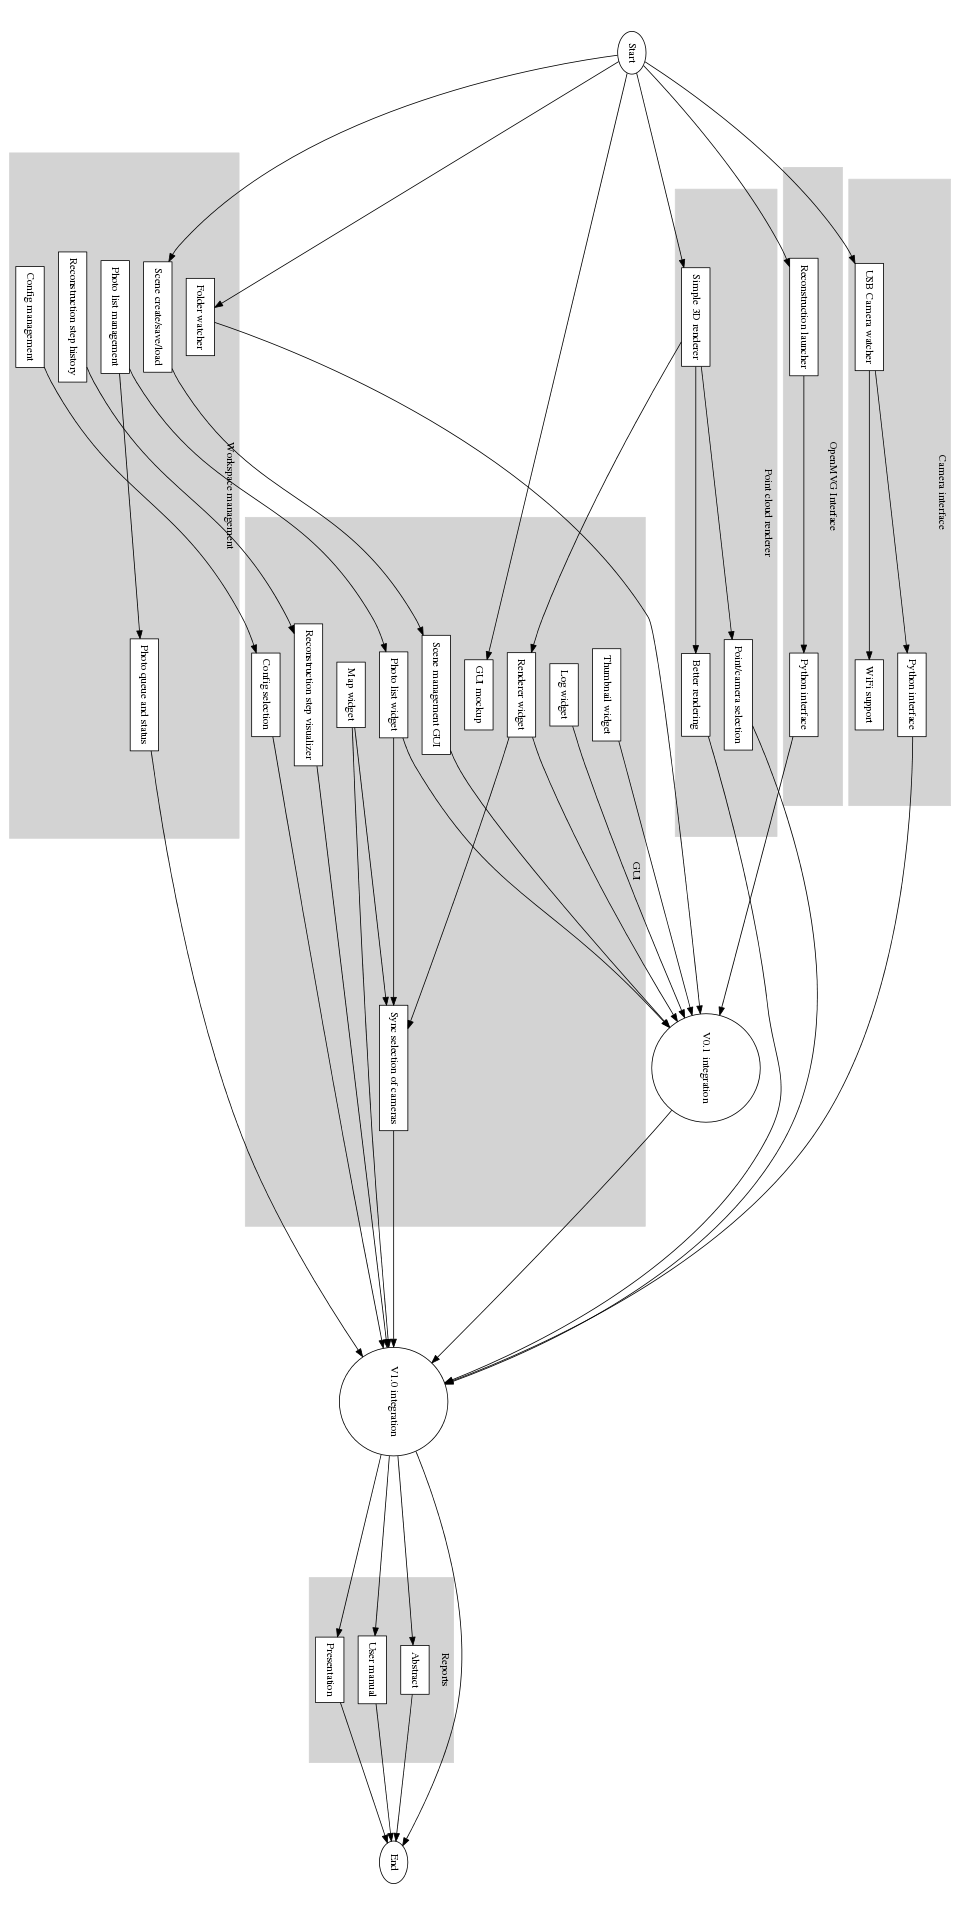
\includegraphics[scale=0.5]{task-dependencies.png}